% \begin{itemize}
%     \item self-convergence tests (1D bte with specified E field)
%     \item cross-verification results with PIC-dsmc
%     \item glow discharge results
%     \begin{itemize}
%     	\item parametric study fluid and hybrid models under different pressure values. 
%		%\item can we describe the differences with drift diffusion approx. differences
%     \end{itemize}
% \end{itemize}
We organize the results as follows. \Cref{subsec:results_specified_E} presents a self-convergence study for the developed Eulerian BTE solver and cross-verification comparison with an in-house PIC-DSMC code. Performance evaluation of the developed algorithms is presented in~\Cref{subsec:peformance_glowd}. \Cref{subsec:results_glowd} presents a detailed comparison study between the hybrid and the fluid approximations of RF-GDPs for different pressure regimes. 

\subsection{Boltzmann transport with specified electric field}
\label{subsec:results_specified_E}

\begin{figure}[!tbhp]
	\begin{center}
		\subfloat[\hspace{-0.7in} \label{fig:case1_1_1}]{
			\begin{tikzpicture}
				\begin{semilogyaxis}[xlabel={$\hat{x}$}, ylabel={$n_e$ electron number density $[\text{m}^{-3}]$}, grid=major, width = 0.32\textwidth,height=0.33\textwidth, legend pos=south west, title style={at={(0.5,1.1)},anchor=north}, title={t=0.2T}]
					\addplot[-, a1, very thick] table[x={x}, y expr=\thisrow{ne} * 8e16 ] {dat/1dbte_with_E/Ewt_10K_Nx100_Nr127_l2_dt_5e-4_02.csv};
					\addplot[-, a2, very thick] table[x={x}, y expr=\thisrow{ne} * 8e16 ] {dat/1dbte_with_E/Ewt_10K_Nx200_Nr255_l4_dt_2e-4_02.csv};
					\addplot[-, a3, very thick] table[x={x}, y expr=\thisrow{ne} * 8e16 ] {dat/1dbte_with_E/Ewt_10K_Nx200_Nr511_l8_dt_1e-4_02.csv};
					\legend{$r_0$, $r_1$, $r_2$};
				\end{semilogyaxis}
		\end{tikzpicture}}
		\subfloat[\hspace{-0.7in}\label{fig:case1_1_2}]{
			\begin{tikzpicture}
				\begin{semilogyaxis}[xlabel={$\hat{x}$}, ylabel={$n_e$ electron number density $[\text{m}^{-3}]$}, grid=major, width = 0.32\textwidth,height=0.33\textwidth, legend pos=north west, title style={at={(0.5,1.1)},anchor=north}, title={t=0.4T}]
					\addplot[-, a1, very thick] table[x={x}, y expr=\thisrow{ne} * 8e16 ] {dat/1dbte_with_E/Ewt_10K_Nx100_Nr127_l2_dt_5e-4_04.csv};
					\addplot[-, a2, very thick] table[x={x}, y expr=\thisrow{ne} * 8e16 ] {dat/1dbte_with_E/Ewt_10K_Nx200_Nr255_l4_dt_2e-4_04.csv};
					\addplot[-, a3, very thick] table[x={x}, y expr=\thisrow{ne} * 8e16 ] {dat/1dbte_with_E/Ewt_10K_Nx200_Nr511_l8_dt_1e-4_04.csv};
					%\legend{$r_0$, $r_1$, $r_2$};
				\end{semilogyaxis}
		\end{tikzpicture}}
		\subfloat[\hspace{-0.7in}\label{fig:case1_1_3}]{
			\begin{tikzpicture}
				\begin{semilogyaxis}[xlabel={$\hat{x}$}, ylabel={$n_e$ electron number density $[\text{m}^{-3}]$}, grid=major,width = 0.32\textwidth,height=0.33\textwidth, legend pos=north west, title style={at={(0.5,1.1)},anchor=north}, title={t=1.0T}]
					\addplot[-, a1, very thick] table[x={x}, y expr=\thisrow{ne} * 8e16 ] {dat/1dbte_with_E/Ewt_10K_Nx100_Nr127_l2_dt_5e-4_10.csv};
					\addplot[-, a2, very thick] table[x={x}, y expr=\thisrow{ne} * 8e16 ] {dat/1dbte_with_E/Ewt_10K_Nx200_Nr255_l4_dt_2e-4_10.csv};
					\addplot[-, a3, very thick] table[x={x}, y expr=\thisrow{ne} * 8e16 ] {dat/1dbte_with_E/Ewt_10K_Nx200_Nr511_l8_dt_1e-4_10.csv};
					%\legend{$r_0$, $r_1$, $r_2$};
				\end{semilogyaxis}
		\end{tikzpicture}}
		
		\subfloat[\hspace{-0.7in}\label{fig:case1_2_1}]{
			\begin{tikzpicture}
				\begin{semilogyaxis}[xlabel={$\hat{x}$}, ylabel= $n_e$ relative error, grid=major,width = 0.32\textwidth,height=0.4\textwidth, legend pos=south west]
					\addplot[-, a1, very thick] table[x={x}, y expr=\thisrow{ne} ] {dat/1dbte_with_E/Ewt_10K_Nx100_Nr127_l2_dt_5e-4_rel_error_02.csv};
					\addplot[-, a2, very thick] table[x={x}, y expr=\thisrow{ne} ] {dat/1dbte_with_E/Ewt_10K_Nx200_Nr255_l4_dt_2e-4_rel_error_02.csv};
					%\addplot[-, a3, very thick] table[x={x}, y expr=\thisrow{ne} ] {dat/1dbte_with_E/Ewt_10K_Nx200_Nr511_l8_dt_1e-4_rel_error_02.csv};
					\legend{$r_0$ vs. $r_2$, $r_1$ vs. $r_2$};
				\end{semilogyaxis}
		\end{tikzpicture}}
		\subfloat[\hspace{-0.7in}\label{fig:case1_2_2}]{
			\begin{tikzpicture}
				\begin{semilogyaxis}[xlabel={$\hat{x}$}, ylabel= $n_e$ relative error, grid=major,width = 0.32\textwidth,height=0.4\textwidth, legend pos=north west]
					\addplot[-, a1, very thick] table[x={x}, y expr=\thisrow{ne} ] {dat/1dbte_with_E/Ewt_10K_Nx100_Nr127_l2_dt_5e-4_rel_error_04.csv};
					\addplot[-, a2, very thick] table[x={x}, y expr=\thisrow{ne} ] {dat/1dbte_with_E/Ewt_10K_Nx200_Nr255_l4_dt_2e-4_rel_error_04.csv};
					%\addplot[-, a3, very thick] table[x={x}, y expr=\thisrow{ne} ] {dat/1dbte_with_E/Ewt_10K_Nx200_Nr511_l8_dt_1e-4_rel_error_04.csv};
					%\legend{$r_0$, $r_1$, $r_2$};
				\end{semilogyaxis}
		\end{tikzpicture}}
		\subfloat[\hspace{-0.7in}\label{fig:case1_2_3}]{
			\begin{tikzpicture}
				\begin{semilogyaxis}[xlabel={$\hat{x}$}, ylabel= $n_e$ relative error, grid=major,width = 0.32\textwidth,height=0.4\textwidth, legend pos=north west]
					\addplot[-, a1, very thick] table[x={x}, y expr=\thisrow{ne} ] {dat/1dbte_with_E/Ewt_10K_Nx100_Nr127_l2_dt_5e-4_rel_error_10.csv};
					\addplot[-, a2, very thick] table[x={x}, y expr=\thisrow{ne} ] {dat/1dbte_with_E/Ewt_10K_Nx200_Nr255_l4_dt_2e-4_rel_error_10.csv};
					%\addplot[-, a3, very thick] table[x={x}, y expr=\thisrow{ne} ] {dat/1dbte_with_E/Ewt_10K_Nx200_Nr511_l8_dt_1e-4_rel_error_10.csv};
					%\legend{$r_0$, $r_1$, $r_2$};
				\end{semilogyaxis}
		\end{tikzpicture}}
		
		\subfloat[\hspace{-0.7in}\label{fig:case1_3_1}]{
			\begin{tikzpicture}
				\begin{semilogyaxis}[xlabel={$e$-energy [eV]}, ylabel= {$f_0$ [$\text{eV}^{-3/2}$]}, grid=major,width = 0.3\textwidth,height=0.4\textwidth, legend pos=north east, title style={at={(0.5,1.1)},anchor=north}, title={t=0.2T, $\hat{x}$=-0.988}]
					\addplot[-, a1, very thick] table[x={x}, y expr=abs(\thisrow{f0}) ] {dat/1dbte_with_E/Ewt_10K_Nx100_Nr127_l2_dt_5e-4_fl_x-0.988_02.csv};
					\addplot[-, a2, very thick] table[x={x}, y expr=abs(\thisrow{f0}) ] {dat/1dbte_with_E/Ewt_10K_Nx200_Nr255_l4_dt_2e-4_fl_x-0.988_02.csv};
					\addplot[-, a3, very thick] table[x={x}, y expr=abs(\thisrow{f0}) ] {dat/1dbte_with_E/Ewt_10K_Nx200_Nr511_l8_dt_1e-4_fl_x-0.988_02.csv};
					\legend{$r_0$, $r_1$, $r_2$};
				\end{semilogyaxis}
		\end{tikzpicture}}
		\subfloat[\hspace{-0.7in}\label{fig:case1_3_2}]{
			\begin{tikzpicture}
				\begin{semilogyaxis}[xlabel={$e$-energy [eV]}, ylabel= {$f_0$ [$\text{eV}^{-3/2}$]}, grid=major,width = 0.3\textwidth,height=0.4\textwidth, legend pos=north east, title style={at={(0.5,1.1)},anchor=north}, title={t=0.4T, $\hat{x}$=-0.988}]
					\addplot[-, a1, very thick] table[x={x}, y expr=abs(\thisrow{f0}) ] {dat/1dbte_with_E/Ewt_10K_Nx100_Nr127_l2_dt_5e-4_fl_x-0.988_04.csv};
					\addplot[-, a2, very thick] table[x={x}, y expr=abs(\thisrow{f0}) ] {dat/1dbte_with_E/Ewt_10K_Nx200_Nr255_l4_dt_2e-4_fl_x-0.988_04.csv};
					\addplot[-, a3, very thick] table[x={x}, y expr=abs(\thisrow{f0}) ] {dat/1dbte_with_E/Ewt_10K_Nx200_Nr511_l8_dt_1e-4_fl_x-0.988_04.csv};
					%\legend{$r_0$, $r_1$, $r_2$};
				\end{semilogyaxis}
		\end{tikzpicture}}
		\subfloat[\hspace{-0.7in}\label{fig:case1_3_3}]{
			\begin{tikzpicture}
				\begin{semilogyaxis}[xlabel={$e$-energy [eV]}, ylabel= {$f_0$ [$\text{eV}^{-3/2}$]}, grid=major,width = 0.3\textwidth,height=0.4\textwidth, legend pos=north east, title style={at={(0.5,1.1)},anchor=north}, title={t=1.0T, $\hat{x}$=-0.988}, xmax=25]
					\addplot[-, a1, very thick] table[x={x}, y expr=abs(\thisrow{f0}) ] {dat/1dbte_with_E/Ewt_10K_Nx100_Nr127_l2_dt_5e-4_fl_x-0.988_10.csv};
					\addplot[-, a2, very thick] table[x={x}, y expr=abs(\thisrow{f0}) ] {dat/1dbte_with_E/Ewt_10K_Nx200_Nr255_l4_dt_2e-4_fl_x-0.988_10.csv};
					\addplot[-, a3, very thick] table[x={x}, y expr=abs(\thisrow{f0}) ] {dat/1dbte_with_E/Ewt_10K_Nx200_Nr511_l8_dt_1e-4_fl_x-0.988_10.csv};
					%\legend{$r_0$, $r_1$, $r_2$};
				\end{semilogyaxis}
		\end{tikzpicture}}
		
		% \subfloat[\hspace{-0.7in}\label{fig:case1_4_1}]{
			% \begin{tikzpicture}
				%     \begin{semilogyaxis}[xlabel=energy $(\text{eV})$, ylabel= $f_1$ ($\text{eV}^{-3/2}$), grid=major,width = 0.33\textwidth,height=0.33\textwidth, legend pos=north east]
					%     \addplot[-, a1, very thick] table[x={x}, y expr=abs(\thisrow{f1}) ] {dat/1dbte_with_E/Ewt_10K_Nx100_Nr127_l2_dt_5e-4_fl_x-0.988_02.csv};
					%     \addplot[-, a2, very thick] table[x={x}, y expr=abs(\thisrow{f1}) ] {dat/1dbte_with_E/Ewt_10K_Nx200_Nr255_l4_dt_2e-4_fl_x-0.988_02.csv};
					%     \addplot[-, a3, very thick] table[x={x}, y expr=abs(\thisrow{f1}) ] {dat/1dbte_with_E/Ewt_10K_Nx200_Nr511_l8_dt_1e-4_fl_x-0.988_02.csv};
					%     \legend{$r_0$, $r_1$, $r_2$};
					%     \end{semilogyaxis}
				% \end{tikzpicture}}
		% \subfloat[\hspace{-0.7in}\label{fig:case1_4_2}]{
			% \begin{tikzpicture}
				%     \begin{semilogyaxis}[xlabel=energy $(\text{eV})$, ylabel= $f_1$ ($\text{eV}^{-3/2}$), grid=major,width = 0.33\textwidth,height=0.33\textwidth, legend pos=north east]
					%     \addplot[-, a1, very thick] table[x={x}, y expr=abs(\thisrow{f1}) ] {dat/1dbte_with_E/Ewt_10K_Nx100_Nr127_l2_dt_5e-4_fl_x-0.988_04.csv};
					%     \addplot[-, a2, very thick] table[x={x}, y expr=abs(\thisrow{f1}) ] {dat/1dbte_with_E/Ewt_10K_Nx200_Nr255_l4_dt_2e-4_fl_x-0.988_04.csv};
					%     \addplot[-, a3, very thick] table[x={x}, y expr=abs(\thisrow{f1}) ] {dat/1dbte_with_E/Ewt_10K_Nx200_Nr511_l8_dt_1e-4_fl_x-0.988_04.csv};
					%     %\legend{$r_0$, $r_1$, $r_2$};
					%     \end{semilogyaxis}
				% \end{tikzpicture}}
		% \subfloat[\hspace{-0.7in}\label{fig:case1_4_3}]{
			% \begin{tikzpicture}
				%     \begin{semilogyaxis}[xlabel=energy $(\text{eV})$, ylabel= $f_1$ ($\text{eV}^{-3/2}$), grid=major,width = 0.33\textwidth,height=0.33\textwidth, legend pos=north east]
					%     \addplot[-, a1, very thick] table[x={x}, y expr=abs(\thisrow{f1}) ] {dat/1dbte_with_E/Ewt_10K_Nx100_Nr127_l2_dt_5e-4_fl_x-0.988_10.csv};
					%     \addplot[-, a2, very thick] table[x={x}, y expr=abs(\thisrow{f1}) ] {dat/1dbte_with_E/Ewt_10K_Nx200_Nr255_l4_dt_2e-4_fl_x-0.988_10.csv};
					%     \addplot[-, a3, very thick] table[x={x}, y expr=abs(\thisrow{f1}) ] {dat/1dbte_with_E/Ewt_10K_Nx200_Nr511_l8_dt_1e-4_fl_x-0.988_10.csv};
					%     %\legend{$r_0$, $r_1$, $r_2$};
					%     \end{semilogyaxis}
				% \end{tikzpicture}}
	\end{center}
	\caption{Electron transport using BTE with specified electric field $E(x,t)=10^4 \sin(2\pi \zeta t)$ with $\zeta=13.56$MHz. \Cref{fig:case1_1_1,fig:case1_1_2,fig:case1_1_3} show the electron number density $n_e(x)=\int_{\vect{v}} f\of{x, \vect{v}}\diff{\vect{x}}$ evolution in time for runs $r_0$, $r_1$, and $r_2$ specified in \Cref{tab:refinement_params}. \Cref{fig:case1_2_1,fig:case1_2_2,fig:case1_2_3} show relative error in $n_e(x)$ with respect to the highest resolution run $r_2$. \Cref{fig:case1_3_1,fig:case1_3_2,fig:case1_3_3} show the electron energy density function at spatial location $\of{2x/L-1}=\hat{x} = -0.988$ for subsequent runs $r_0$, $r_1$ and $r_2$.\label{fig:self_convegence_1d_bte_with_E}}
\end{figure}

We consider the electron BTE with zero incoming flux boundary conditions as specified by~\Cref{eq:hybrid_cnt_b,eq:hybrid_cnt_b_bdy}.
%\begin{subequations}
%    \begin{align}
%        &\partial_t f + v\cos\of{\vtheta} \partial_x f- \frac{q_e E}{m_e} \of{\cos(\vtheta) \partial_v f - \sin(\vtheta) \frac{1}{v} \partial_{\vtheta}f } = C_{en}(f) \text{ for } x \in [0, L]\label{eq:bte_1d_1}, 
%        \\
%        &f(x=0, v, \vtheta \leq \frac{\pi}{2}, \vphi) = 0 \text{ and } f(x=L, v, \vtheta > \frac{\pi}{2}, \vphi) = 0 \label{eq:1d_bte_bc_1}. 
%        %&\vect{E}\of{x,t} = E_0  \sin\of{2\pi f t} \label{eq:bte_with_E_field}. %\of{\frac{2x}{L}-1}^a
%    \end{align}\label{eq:bte_with_E}
%\end{subequations}

We evolve this equation with the initial conditions described by
\begin{align}
    &f(t=0, x, \vect{v}) = \frac{n_e\of{t=0, x}}{{\pi}^{3/2}v_{th}^3} \exp\of{-\of{\frac{\norm{\vect{v}}_2}{v_{th}}}^2} \nonumber \text{ where, } \\ 
    n_e\of{t=0, x} &= 10^{13} + 10^{15} (1- x / L)^2 (x/L)^2 \ [\text{m}^{-3}] \text { ,  } v_{th} = \sqrt{\frac{2k_B T_e}{m_e}} \text{ and } T_e = 0.5 \text{eV}\label{eq:ic_liu},
\end{align} with a specified electric field $E(x,t)$. The electric field causes electron acceleration along the opposite direction, triggering ionization events. Hence, we observe oscillatory growth of electron number density. 

\textit{Convergence}: We use this problem to perform a convergence study. We consider a time-harmonic spatially homogeneous electric field given by $E(x, t) = 10^4 \sin(2\pi \zeta t)$ [V/m] with $\zeta$ = 13.56MHz. \Cref{tab:refinement_params} summarizes the parameters used for the convergence study. \Cref{fig:self_convegence_1d_bte_with_E} shows the convergence of the evolved solution with increasing resolution in the phase space.  \Cref{fig:case1_1_1,fig:case1_1_2,fig:case1_1_3} show the oscillatory growth of the electron number density $n_e(x)$, \Cref{fig:case1_2_1,fig:case1_2_2,fig:case1_2_3} show the relative errors of $n_e(x)$ with respect to the highest resolution run, and \Cref{fig:case1_3_1,fig:case1_3_2,fig:case1_3_3} show the convergence of the electron energy density function at a chosen spatial location. 
\begin{table}[!tbhp]
    \centering
    \begin{tabular}{|c|c|c|c|c|c|}
        \hline
        run id & $N_x$ & $N_r$ & $N_{\vtheta}$ & $N_{l}$ & $\frac{\Delta t}{(1/\zeta)}$ \\
        \hline
        $r_0$ & 100 & 128 & 16 & 2 & 5e-4 \\
        $r_1$ & 200 & 256 & 32 & 4 & 2e-4 \\
        $r_2$ & 200 & 512 & 64 & 8 & 1e-4 \\
        \hline 
    \end{tabular}
    \caption{Refinement parameters used in space, velocity space and time for the convergence study presented in \Cref{fig:self_convegence_1d_bte_with_E}. \label{tab:refinement_params}}
\end{table}

\begin{figure}[!tbhp]
	\begin{center}
		\begin{tikzpicture}
			\begin{semilogyaxis}[xlabel= {$\hat{x} = \frac{2x}{L} - 1$}, ylabel= {number density $[\text{m}^{-3}]$}, grid=major,width = 0.48\textwidth,height=0.46\textwidth, legend pos=south east]
				\addplot[        dotted, a1, very thick]  table[x={x}, y expr=\thisrow{ne_pde} ] {dat/1dbte_with_E_pic_vs_pde/Ewt_10K_pde_idx_0000.csv};
				\addplot[        -     , a2, very thick]  table[x={x}, y expr=\thisrow{ne_pde} ] {dat/1dbte_with_E_pic_vs_pde/Ewt_10K_pde_idx_0010.csv};
				\addplot[        dashed, a3, very thick]  table[x={x}, y expr=\thisrow{ne_pic} ] {dat/1dbte_with_E_pic_vs_pde/Ewt_10K_pic_idx_0010.csv};
				\legend{initial condition, \bte, PIC-DSMC};
			\end{semilogyaxis}
		\end{tikzpicture}
		\begin{tikzpicture}
			\begin{axis}[xlabel = {$\hat{x} = \frac{2x}{L} - 1$}, ylabel= {temperature [eV]}, grid=major,width = 0.48\textwidth,height=0.46\textwidth, legend pos=south east]
				\addplot[        dotted, a1, very thick]  table[x={x}, y expr=\thisrow{Te_pde} ] {dat/1dbte_with_E_pic_vs_pde/Ewt_10K_pde_idx_0000.csv};
				\addplot[        -     , a2, very thick]  table[x={x}, y expr=\thisrow{Te_pde} ] {dat/1dbte_with_E_pic_vs_pde/Ewt_10K_pde_idx_0010.csv};
				\addplot[        dashed, a3, very thick]  table[x={x}, y expr=\thisrow{Te_pic} ] {dat/1dbte_with_E_pic_vs_pde/Ewt_10K_pic_idx_0010.csv};
				%\legend{initial condition, Eulerian, PIC-DSMC};
			\end{axis}
		\end{tikzpicture}
	\end{center}
	\caption{We consider the electron BTE given in \Cref{eq:hybrid_cnt_b,eq:hybrid_cnt_b_bdy} with electric field $E(x,t)=10^4 \sin(2\pi \zeta t)$ with $\zeta=13.56$MHz. The figure shows solutions after a one period 1/f. The blue line is~\bte~and the broken green line is PIC-DSMC. \label{fig:case1_pic_vs_pde}}
\end{figure}

We solve the electron BTE given in \Cref{eq:hybrid_cnt_b,eq:hybrid_cnt_b_bdy} with our \bte~and PIC-DSMC codes and we report the results in \Cref{fig:case1_pic_vs_pde}. The results show excellent agreement between the two solvers. 
%In the above, the solutions computed using Eulerian and PIC-DSMC approaches show excellent agreement. 

\subsection{Performance evaluation}
\label{subsec:peformance_glowd}
We summarize performance evaluation results for the fluid and \bte~solvers for RF-GDPs. We conducted our experiments on Lonestar 6 at the Texas Advanced Computing Center (TACC). Each node on Lonestar 6 has two AMD EPYC 7763 CPUs and three NVIDIA A100 GPUs. 
\begin{table}[!tbhp]
	\centering
	\begin{tabular}{||c|c|c||}
		\hline
		$N_x$ & $\Delta t / (1/\zeta) $  & timestep (s) \\
		\hline
		100	  & 1.00E-03        & 9.0785E-03 \\
		200	  & 1.00E-03        & 2.9685E-02 \\
		400	  & 1.00E-03        & 1.7288E-01 \\
		\hline
	\end{tabular}
	\caption{The fluid solver runtime for a single implicit timestep with increasing spatial resolution. The above results are conducted using a single core of AMD EPYC 7763 CPU \label{tab:performance_fluid}.}
\end{table}
The presented fluid and \bte~performance results are conducted on a single AMD EPYC 7763 CPU core and a single NVIDIA A100 GPU. \Cref{tab:performance_fluid} summarizes the overall implicit timestep cost for the fluid solver. We observe $\mathcal{O}(N_x^3)$ growth of the timestep cost where $N_x$ denotes the number of Chebyshev collocation points in space. This is due to the direct Jacobian factorization used in the Newton iteration. 

Performance evaluation results of the \bte~solver is presented in \Cref{tab:performance_hybrid}. 
\begin{table}[!tbhp]
	\centering
	\resizebox{\textwidth}{!}{
		\begin{tabular}{||c|c|c|c|c|c|c|c|c||}
			\hline
			$N_r$ & $N_\vtheta$ & $N_l$ & $N_x$ & $\Delta t_S \times f$ & $\Delta t_F \times f$ & semi-implicit (s) & fully-implicit (s) & speedup\\
			\hline
			64  & 16 & 3 & 100 & 5E-05 & 2E-04 & 3.53E-02 &  6.52E-02 & 2.1x\\
			128 & 16 & 3 & 100 & 5E-05 & 2E-04 & 3.61E-02 &  6.55E-02 & 2.2x\\
			256 & 16 & 3 & 100 & 5E-05 & 2E-04 & 3.71E-02 &  6.68E-02 & 2.2x\\
			\hline
			\hline
			64  & 16 & 3 & 100 & 5E-05 & 2E-04 & 3.53E-02 &  6.52E-02 & 2.1x\\
			128 & 16 & 3 & 200 & 5E-05 & 2E-04 & 3.93E-02 &  2.52E-01 & 0.6x \\
			256 & 16 & 3 & 400 & 5E-05 & 2E-04 & 6.37E-02 &  --& --\\
			\hline
	\end{tabular}}
	\caption{Comparison of the overall timestep cost for the \bte~solver using semi-implicit and fully-implicit schemes. Although the fully implicit solver is more expensive per timestep, it is faster overall because it requires fewer timesteps. The last column shows the overall runtime (semi-implicit / fully-implicit). The fully-implicit scheme is $\sim2\times$ faster than the semi-implicit scheme for coarser spatial grids $N_x$=100. For $N_x\geq 200$ the fully-implicit solve becomes too expensive.
		%The efficiency $S$ of the fully-implicit scheme reduces with increasing spatial resolution $N_x \geq $ 200
		\label{tab:performance_hybrid}}
\end{table}
Here, $N_x$, $N_r$, $N_\vtheta$, and $N_l$ denote the number of Chebyshev collocation points in the position space, B-spline basis functions in speed, discrete ordinate points, and spherical basis functions are used in $\vtheta$. For coarser spatial grids, we observe that the fully-implicit scheme is $\sim 2\times$ faster than the semi-implicit scheme. With increased spatial resolution, the fully-implicit scheme becomes more expensive than the semi-implicit scheme. This is primarily due to the increased $T_{\vect{x}\text{-rhs}}$ cost. Recall that the  complexities of fully-implicit and semi-implicit schemes are given by $2k(T_{\vect{x}\text{-rhs}} + T_{\vect{v}\text{-rhs}})$ and $(T_{\vect{x}\text{-rhs}} + 2k T_{\vect{v}\text{-rhs}})$ where $k$ denotes the number of iterations for convergence. Hence, the increased $T_{\vect{x}\text{-rhs}}$ reduces the overall efficiency of the fully-implicit scheme. Of course both methods are orders of magnitude faster than an explicit method. We use the coarse grid fully-implicit scheme to march over the transient and reach the time-periodic state. Once time-periodicity is reached, we use iterative refinement with semi-implicit time integration to resolve the finer features of the time-periodic state.

\Cref{fig:cost_breakdown} shows the overall cost breakdown for a single timestep for evolving the hybrid formulation of RF-GDPs with semi-implicit and fully-implicit time integration schemes. We compute these percentages based on each method's overall runtime for a single complete timestep to evolve ions and electrons. Even though the relative cost of the BTE update is 10\% higher in the fully-implicit scheme, compared to the semi-implicit approach, it allows larger timestep sizes that respect timescales of ions. 
\begin{figure}[!tbhp]
	\centering
	\small
	\resizebox{\textwidth}{!}{
	\begin{tabular}{cc}
		\textbf{Semi-implicit} & \textbf{Fully-implicit}\\
		\begin{tikzpicture}
			\pie[radius=1.5, text=pin,color={blue!50,red!50}]{18.6/\text{Solve (ions-fluid)}, 80.34/\text{Solve (e-BTE)}};
		\end{tikzpicture} & \begin{tikzpicture}
			\pie[radius=1.5,text=pin, color={blue!50,red!50}]{10.41/\text{Solve (ions-fluid)}, 89.04/\text{Solve (e-BTE)}};
		\end{tikzpicture}\\
	$(N_r,N_x,N_l,N_{\vtheta}, \Delta t \times f)=(256, 100, 3, 16, \text{5E-5})$ & $(N_r,N_x,N_l,N_{\vtheta}, \Delta t \times f)=(256, 100, 3, 16, \text{2E-4 })$\\
	\end{tabular}}
\caption{The overall runtime cost breakdown for a single RF-GDP timestep using the hybrid modeling approach. The left and right plots show the cost breakdown using semi-implicit and fully-implicit schemes for evolving the electron BTE. In both cases, $\vect{E}$-field solve cost is negligible compared to others, hence omitted in the plot. \label{fig:cost_breakdown}}
\end{figure}


\subsection{Glow discharge}
\label{subsec:results_glowd}
For modeling RF-GDPs, we present a comparative study of the fluid and the hybrid approaches, which are given by~\Cref{eq:fluid_model_eqs,eq:glow_hybrid}. The key difference between the fluid and hybrid modeling approaches is how the electron transport is being modeled. The fluid approach transports electrons and ions using fluid equations. In contrast, in the hybrid model, electron transport is kinetic by solving the BTE, while we use the standard fluid transport for ions. We consider four cases with varying gas pressure values ranging from 0.1 Torr to 2 Torr while keeping other parameters unchanged. Since $n_0 \sim \frac{p_0}{k_B T}$, lower pressure values result in lower background number densities. This causes the plasma to be less collisional. Our primary goal is to identify the modeling discrepancies between hybrid and fluid-based electron transport under different pressure regimes. The simulation parameters used for the study are summarized in \Cref{t:model_parameters}. 
\begin{table}[!tbhp]
	\centering
	\resizebox{\textwidth}{!}{
	\begin{tabular}{|c|c|c|c|}
		\hline 
		\hline
		Parameter & Symbol &  Value & Reference \\
		\hline
		\small Gas pressure     & $p_0$ & 0.1Torr, 0.5Torr, 1Torr, 2Torr  & --\\
		\small Gas temperature  & $T_0$ & 300 K & --\\
		\small Neutral density  & $n_0$ & (0.322, 1.61, 3.22, 6.44)$\times 10^{22} \text{m}^{-3}$  & ideal gas law\\
		\small Electrode gap    & $L$   & 2.54 $\times 10^{-2}$ $\text{m}$ & \cite{liu2014numerical}\\
		\small Peak voltage     & $V_0$ & 100 V & \cite{liu2014numerical} \\
		\small Oscillation frequency & $f$ & 13.56 MHz & \cite{lymberopoulos1993fluid}\\
		\small Electron diffusion  & $D_e$  & \bolsig~ (0D-BTE) & \cite{hagelaar2005solving, hagelaar2015coulomb}\\
		\small Ion diffusion   & $D_i$ & $n_0 D_i = 2.07 \times 10^{20} \text{m}^{-1}\text{s}^{-1}$ & \cite{lymberopoulos1993fluid} \\
		\small Electron mobility  & $\mu_e$ & \bolsig~ (0D-BTE) & \cite{hagelaar2005solving, hagelaar2015coulomb}\\
		\small Ion mobility    & $\mu_i$ & $n_0 \mu_i = 4.65 \times 10^{21} \text{V}^{-1}\text{m}^{-1}\text{s}^{-1}$ & \cite{lymberopoulos1993fluid}\\
		\small $e + Ar \rightarrow 2e + Ar^{+}$ & $k_i$ & \bolsig~ (0D-BTE) & \cite{hagelaar2005solving, hagelaar2015coulomb}\\
		\hline
		\hline
	\end{tabular}}
	\caption{Modeling parameters used in the presented work. \label{t:model_parameters}}
\end{table}
The fluid approximation-based species transport relies on a closure model for kinetic coefficients. The simplest closure model would be the Maxwellian EDF assumption and derive temperature-based electron kinetic coefficients~\cite{liu2014numerical}. The above is not ideal due to the electric field effects in RF-GDPs and other LTPs because of strong deviation from Maxwellian and non-local effects that can occurs at low pressures. In our fluid approximation, we allow non-Maxwellian treatment of kinetic coefficients by solving spatially homogeneous electron BTE. We use the state-of-the-art \bolsig~framework~\cite{hagelaar2005solving} to compute steady-state EDFs for varying $\norm{\vect{E}}$ values with corresponding neutral density $n_0$ and gas temperature $T_0$. With the computed steady-state EDFs, we build electron temperature-based look-up tables for required electron kinetics. The above process is illustrated in \Cref{fig:tab_kinetics_process}. \Cref{fig:bte_0d_kinetics} shows the tabulated kinetic coefficients plotted against the electron temperature $T_e$. Following~\cite{liu2014numerical} we use constant $D_i$, $\mu_i$ for ions. 
%For heavy species transport, we use constant kinetic coefficients similar to ~\cite{liu2014numerical}.

\begin{figure}[!tbhp]
	\centering
	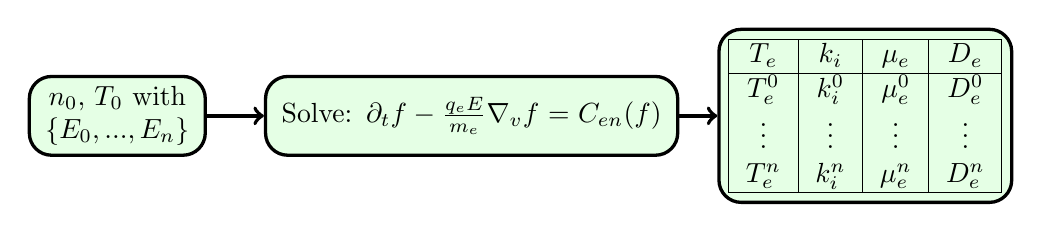
\begin{tikzpicture}
		\tikzstyle{d}=[rectangle,
		rounded corners=8pt,
		very thick,
		text centered,
		minimum size=1cm,
		draw=black!100,
		fill=green!10];
		\node[text width=2cm, d](A) at (0,0) {$n_0$, $T_0$ with $\{E_0, ..., E_{n}\}$};
		\node[text width=5cm, d](B) at (4.5,0) {Solve: $\partial_t f - \frac{q_eE}{m_e} \nabla_{\vect{v}} f = C_{en}(f)$};
		\node[d](C) at (9.5, 0)
		{		
				\begin{tabular}{|c|c|c|c|}
					\hline
					$T_e$ & $k_i$ & $\mu_e$ & $D_e$\\
					\hline
					$T_e^0$ & $k_i^0$ & $\mu_e^{0}$ & $D_e^{0}$ \\
					\vdots & \vdots& \vdots & \vdots\\
					$T_e^n$ & $k_i^n$ & $\mu_e^{n}$ & $D_e^{n}$ \\
					\hline
				\end{tabular}
		};
	\draw[->, line width=0.5mm] (A) -- (B);
	\draw[->, line width=0.5mm] (B) -- (C);
	\end{tikzpicture}
\caption{An illustrative diagram that describes the process of computing tabulated kinetic coefficients for electrons to be used in the fluid model (Equation~\ref{eq:fluid_model_eqs}). For a fixed $n_0$, $T_0$, we compute the steady-state EDF solutions for the spatially homogeneous BTEs for a given electric field values i.e., $\{E_0,...,E_n\}$. For each $E_j$, we compute kinetic coefficients \{$k_i^j$, $\mu_e^j$, $D_e^j$\} and corresponding temperature $T_e^j$. Then for example, for $\mu_e$, we build an interpolant $\mu_e(T_e)$ using the $\{\mu_e^j, T_e^j\}$ pairs. 
%This will result in electron kinetic coefficients (i.e., $k_i$, $\mu_e$, and $D_e$) for the corresponding steady-state electron temperature $T_e$ values (i.e., $\{T_e^{0},...,T_e^{n}\}$). We use the above to build electron temperature-based tabulated kinetic coefficients that are used in the fluid approximation.
\label{fig:tab_kinetics_process} 
}
\end{figure}

\begin{figure}[!tbhp]
	\centering
	\begin{tikzpicture}
		\begin{semilogyaxis}[xlabel={temperature [eV]}, ylabel={ionization rate $[m^3s^{-1}]$}, grid=major, width = 0.32\textwidth, height=0.33\textwidth, ymin=1e-28]
			\addplot[blue, very thick] table[x expr = \thisrow{Te(K)}/11604.518, y expr=1e-100 + \thisrow{kf(m3/s)}, col sep=comma]{dat/Ar_1Torr_300K/Ionization.300K.txt};
		\end{semilogyaxis}
	\end{tikzpicture}
	\begin{tikzpicture}
		\begin{semilogxaxis}[xlabel={temperature [eV]}, ylabel= $D_e (m^{2}s^{-1})$ $\rightarrow$, grid=major, width = 0.32\textwidth, height=0.33\textwidth]
			\addplot[blue, very thick] table[x expr = \thisrow{Te(K)}/11604.518, y expr = \thisrow{D*N(1/m-s)}/3.22e22, col sep=comma]{dat/Ar_1Torr_300K/Diffusivity.300K.txt};
		\end{semilogxaxis}
	\end{tikzpicture}
	\begin{tikzpicture}
		\begin{loglogaxis}[xlabel={temperature [eV]}, ylabel= $\mu_e (V^{-1} m^{2} s^{-1})$ $\rightarrow$, grid=major,width = 0.32\textwidth, height=0.33\textwidth]
			\addplot[blue, very thick] table[x expr = \thisrow{Te(K)}/11604.518, y expr =\thisrow{Mu*N(1/V-m-s)} / 3.22e22, col sep=comma]{dat/Ar_1Torr_300K/Mobility.300K.txt};
		\end{loglogaxis}
	\end{tikzpicture}
	\caption{Tabulated electron kinetic coefficients based on the steady-state solutions of the 0D3V electron BTE. \label{fig:bte_0d_kinetics}}
\end{figure}

For RF-GDPs, the time-periodic steady-state solution is determined by the background gas temperature $T_0$, pressure $p_0$, the electrode gap $L$, and the peak driving voltage $V_0$. As mentioned, we consider the $p_0$ values listed in \Cref{t:model_parameters} while keeping all other parameters fixed. Changing $p_0$ changes the neutral density $n_0$, which is coupled to the problem through electron-heavy binary collisions and heavy species kinetic coefficients. 

Both hybrid and fluid solvers were time-marched until the time-periodic state is achieved. We compute the time-periodic solution from the fluid solver with initial conditions given by~\cite{lymberopoulos1993fluid}. This solution is then used as an initial condition for the hybrid solver, where the EDFs are initialized as Maxwellian distributions defined by the temperature computed by the fluid solver. %The primary difference between the fluid and the hybrid approaches is the electron transport. 

%We evolve the fluid and hybrid RF-GDP models for the parameters summarized in \Cref{t:model_parameters} until the time-periodic steady-state is achieved. Note that, for the fluid approximation, we allow non-Maxwellian treatment of EDFs through tabulated kinetic coefficients computed by solving spatially homogeneous BTE for local plasma conditions. First, we compute the time-periodic steady-state solution from the fluid solver where the initial conditions are similar to~\cite{lymberopoulos1993fluid}. The time-periodic steady-state solution predicted by the fluid approximation is used as an initial condition for the hybrid solver, where EDFs are initialized for Maxwellian distribution with the local temperature. The key difference between the fluid and hybrid modeling approaches is how the electron transport is being modeled. The fluid approach transports electrons and ions using fluid equations. In contrast, in the hybrid model, electron transport is entirely handled by the BTE, and the fluid approximation handles the transport of ions. 

\begin{figure}[!tbhp]
	\includegraphics[width=\textwidth]{fig/0.1Torr300K_100V_Ar_3sp2r_cycle_qoi.png} \\
	\includegraphics[width=\textwidth]{fig/0.5Torr300K_100V_Ar_3sp2r_cycle_qoi.png} \\
	\includegraphics[width=\textwidth]{fig/1Torr300K_100V_Ar_3sp2r_cycle_qoi.png} \\
	\includegraphics[width=\textwidth]{fig/2Torr300K_100V_Ar_3sp2r_cycle_qoi.png} 
	\caption{Cycle-averaged time-periodic steady-state profiles computed by the hybrid and the fluid approximation of RF-GDPs under varying pressure values from 0.1 Torr to 2 Torr. \label{fig:ca_profiles_fluid_vs_hybrid} }
\end{figure}
\begin{table}[!tbhp]
	\centering
	\resizebox{\textwidth}{!}{
		\begin{tabular}{|c|m{2.3cm}|m{2.3cm}|m{2.3cm}|m{2.3cm}|m{2.3cm}|m{2.3cm}|}
			\hline 
			&  \multicolumn{3}{c|}{\textbf{Hybrid - cycle averaged peak}}  &  \multicolumn{3}{c|}{\textbf{Fluid - cycle averaged peak}} \\
			\hline
			$\bf{p_0}\ [Torr]$ & $\bf{n_e}\ [m^{-3}]$ & $\bf{\varepsilon_e}\ [eV kg m^{-3}]$ & $\bf{|E|}\ [V/m]$ & $\bf{n_e}\ [m^{-3}]$ & $\bf{\varepsilon_e}\ [eV kg m^{-3}]$ & $\bf{|E|}\ [V/m]$\\
			\hline
			0.1 & 4.27E+16 & 5.65E-14 & 2.32E+04 & 5.87E+14 & 3.660E-15 & 1.27E+04 \\
			\hline
			0.5 & 2.51E+16 & 5.33E-14 & 3.15E+04 & 8.18E+15 & 4.35E-14 & 3.23E+04 \\
			\hline
			1.0 & 4.06E+16 & 1.10E-13 & 4.44E+04 & 2.51E+16 & 1.31E-13 & 4.83E+04\\
			\hline
			2.0 & 7.67E+16 & 1.72E-13 & 5.32E+04 & 7.79E+16 & 3.98E-13 & 7.06E+04 \\
			\hline
	\end{tabular}}
	\caption{A summary of the peak values for the cycle-averaged time-periodic steady-state profiles computed by fluid and hybrid modeling approaches. \label{tab:fluid_vs_hybrid}}
\end{table}

The cycle-averaged profiles are shown in \Cref{fig:ca_profiles_fluid_vs_hybrid}. \Cref{tab:fluid_vs_hybrid} summarizes the peak values for the cycle-averaged time-periodic solutions computed by fluid and hybrid models. For the cycle-averaged profiles, the largest discrepancy between the fluid and the hybrid model is reported in the lowest pressure case, $p_0$ = 0.1 Torr. Specifically, the hybrid computed peak cycle-averaged steady-state electron number density is 80x, 3x, and 1.6x higher compared to the equivalent fluid runs for 0.1 Torr, 0.5 Torr, and 1 Torr cases. For the highest pressure case presented, $p_0$ = 2 Torr, the cycle-averaged electron number density profiles agree quite well but there are still discrepancies, for example the peak electric field. Below we list the reasons that contribute to this discrepancies. 
%Due to the non-linearity, and non-local coupling of modeling equations (i.e., both fluid and hybrid approaches) is it not possible to idle a single cause to explain the differences we observe between models, but we can list the following reasons that cumulatively contribute to the observed differences. 

\begin{figure}[!tbhp]
	\includegraphics[width=0.24\textwidth]{fig/0.1Torr300K_100V_Ar_3sp2r_cycle_ki.png} 
	\includegraphics[width=0.24\textwidth]{fig/0.5Torr300K_100V_Ar_3sp2r_cycle_ki.png} 
	\includegraphics[width=0.24\textwidth]{fig/1Torr300K_100V_Ar_3sp2r_cycle_ki.png}   
	\includegraphics[width=0.24\textwidth]{fig/2Torr300K_100V_Ar_3sp2r_cycle_ki.png}   
	\caption{Discrepancies in the ionization rate coefficient computed from the tabulated data generated form steady-state spatially homogeneous BTE and spatially coupled BTE in the hybrid modeling approach. \label{fig:ki_fluid_vs_hybrid}}
\end{figure}

\begin{figure}[!tbhp]
	\centering
	\includegraphics[width=\textwidth]{fig/0.1Torr300K_100V_Ar_3sp2r_cycle_eedf.png}
	\includegraphics[width=\textwidth]{fig/0.5Torr300K_100V_Ar_3sp2r_cycle_eedf.png}
	\includegraphics[width=\textwidth]{fig/1Torr300K_100V_Ar_3sp2r_cycle_eedf.png}
	\includegraphics[width=\textwidth]{fig/2Torr300K_100V_Ar_3sp2r_cycle_eedf.png}
	\caption{Cycle-averaged time-periodic steady-state EDF solutions in RF-GDPs for the different pressure values computed using the hybrid modeling approach. \label{fig:eedf_hybrid}}
\end{figure}

\textbf{Tabulated rate coefficients}: The fluid approximation of the RF-GDPs relies on a closure model for the electron kinetic coefficients. In the fluid solve, electron kinetics are computed using tabulated results using the 0D3V BTE while for hybrid model, kinetics coefficients are computed by the 1D3V BTE. 
%For the presented fluid model, the tabulated kinetic coefficients are constructed by solving a series of spatially homogeneous electron BTEs for steady-state EDFs with varying electric field magnitudes. The above data is used to construct one-dimensional tabulated kinetic coefficients, which are queried by the corresponding steady-state electron temperature. \Cref{fig:ki_fluid_vs_hybrid} shows the ionization rate coefficient computed by the tabulated data with the fluid approximated electron temperature ($T_e^\mathrm{Fluid}$) and using the EDF computed by solving one-dimensional electron BTE in the hybrid modeling approach.
%We observe that, at the sheath, the tabulated rate coefficient computed by using $T_e^\mathrm{Hybrid}$ matches closely with the rate coefficient computed by solving one-dimensional BTE. The above is due to the large electric field presence at the sheath region reduces the relative effect of the spatial coupling terms in the BTE. At the core of the discharge, we observe that the tabulated rate coefficients cannot produce ions with the electron temperature reported by the hybrid model. The above is primarily due to the fact that the spatial coupling effects reduce tail depletion due to collisions, enabling to trigger ionization reactions with a lower core temperature. 
\Cref{fig:eedf_hybrid} shows the radial components of the cycle-averaged steady-state EDFs computed by the hybrid solver. With increasing background gas pressure, the EDFs at the center of the discharge show rapidly depleted tails at the ionization energy threshold value 15.76 eV. Specifically, for the 0.1 Torr case, tails are more prominent due to reduced collisionality. Similarly, the anisotropic correction modes are dominant compared to runs with higher background gas pressure. Furthermore, tabulated data-based kinetic coefficients
are inaccurate for low-pressure cases because the 0D3V BTE misses spatial coupling effects. These effects become more pronounced with decreasing pressure. 

\textbf{The drift-diffusion approximation}: 
The fluid model uses the drift-diffusion approximation to derive a closed expression for the electron flux term $\vect{J}_e$. The drift-diffusion approximation assumes that the EDFs are isotropic and electron drift velocity is negligible compared to the collisional momentum transfer frequency. \Cref{fig:drift_velocity_hybrid_fluid} shows the cycle-averaged electron drift velocity computed by the hybrid and the fluid modeling approaches. At the sheath region, we observe higher relative errors, greater than 1\%, compared to the center. Due to the large electric field effects, the EDFs at the sheath regions depict higher anisotropic effects compared to the discharge center (see \Cref{fig:eedf_hybrid}). Therefore, the drift-diffusion approximation becomes less valid at the sheath regions and has larger errors compared to the discharge center.   

%The presented fluid model uses the drift-diffusion approximation to derive a closed expression for the electron flux term $\vect{J}_e$. The drift-diffusion approximation assumes that the EDFs are isotropic and electron drift velocity is negligible compared to the collisional momentum transfer frequency. \Cref{fig:drift_velocity_hybrid_fluid} shows the electron drift velocity magnitude $\norm{\vect{u}_e}_2$ computed by the hybrid and the fluid modeling approaches. At the sheath region, we observe higher relative errors (i.e., greater than 1\%) compared to the center. Due to the large electric field effects, the EDFs at the sheath regions depict higher anisotropic effects compared to the discharge center (see \Cref{fig:eedf_hybrid}). Therefore, the drift-diffusion approximation becomes less valid at the sheath regions and has larger errors compared to the discharge center.   

\begin{figure}[!tbhp]
	\centering
	%\includegraphics[width=\textwidth]{fig/0.1Torr300K_100V_Ar_3sp2r_cycle_uz.png} \\
	%\includegraphics[width=\textwidth]{fig/0.5Torr300K_100V_Ar_3sp2r_cycle_uz.png} \\
	%\includegraphics[width=\textwidth]{fig/1Torr300K_100V_Ar_3sp2r_cycle_uz.png}   \\
	%\includegraphics[width=\textwidth]{fig/2Torr300K_100V_Ar_3sp2r_cycle_uz.png}   
	%u_z \caption{Comparison of the electron drift velocity magnitude ($||\vect{u}_e||_2$) computed based on the hybrid and the fluid approximation modeling approaches. The third column shows the relative error between the two approaches taking the hybrid model as the true solution. \label{fig:drift_velocity_hybrid_fluid}}
	
	\includegraphics[width=0.46\textwidth]{fig/0.1Torr300K_100V_Ar_3sp2r_cycle_uz_ca.png} 
	\includegraphics[width=0.46\textwidth]{fig/0.5Torr300K_100V_Ar_3sp2r_cycle_uz_ca.png}
	\includegraphics[width=0.46\textwidth]{fig/1Torr300K_100V_Ar_3sp2r_cycle_uz_ca.png}   
	\includegraphics[width=0.46\textwidth]{fig/2Torr300K_100V_Ar_3sp2r_cycle_uz_ca.png}   
	
	\caption{Comparison of the cycle-averaged electron drift velocity computed based on the hybrid and the fluid approximation modeling approaches. The second column for each case shows the relative error between the two approaches taking the hybrid model as the true solution with respect to its $l_2$ norm. \label{fig:drift_velocity_hybrid_fluid}}
\end{figure}

\textbf{Boundary conditions}: For the hybrid approximation, we use zero incoming flux boundary conditions for the electrons. This will cause non-Maxwellian EDFs at the discharge walls. In contrast, the fluid approximation assumes Maxwellian EDF at discharge walls. Specifically, for the fluid model, the electron boundary flux term is derived based on the Maxwellian EDF assumption, and it is non-linearly coupled to the electron energy equation. The above discrepancy in the boundary EDF between the models also contributes to the differences we observe in the steady-state profiles. 



%\begin{figure}[!tbhp]
%	\centering
%	\includegraphics[width=\textwidth]{fig/0.1Torr300K_100V_Ar_3sp2r_cycle.png} \\
%	\includegraphics[width=\textwidth]{fig/0.5Torr300K_100V_Ar_3sp2r_cycle.png} \\
%	\includegraphics[width=\textwidth]{fig/1Torr300K_100V_Ar_3sp2r_cycle.png}   \\
%	\includegraphics[width=\textwidth]{fig/2Torr300K_100V_Ar_3sp2r_cycle.png}   
%%	\caption{Comparison of the electron drift velocity magnitude ($||\vect{u}_e||_2$) computed based on the hybrid and the fluid approximation modeling approaches. The third column shows the relative error between the two approaches taking the hybrid model as the true solution. \label{fig:drift_velocity_hybrid_fluid}}
%\end{figure}

 




%\begin{figure}[!tbhp]
%	\includegraphics[width=0.99\textwidth]{fig/0.1Torr300K_100V_Ar_3sp2r_cycle.png} \\
%	\includegraphics[width=0.99\textwidth]{fig/0.5Torr300K_100V_Ar_3sp2r_cycle.png} \\
%	\includegraphics[width=0.99\textwidth]{fig/1Torr300K_100V_Ar_3sp2r_cycle.png} \\
%	\includegraphics[width=0.99\textwidth]{fig/2Torr300K_100V_Ar_3sp2r_cycle.png} \\
%\end{figure}



